% Options for packages loaded elsewhere
\PassOptionsToPackage{unicode}{hyperref}
\PassOptionsToPackage{hyphens}{url}
%
\documentclass[
]{book}
\usepackage{lmodern}
\usepackage{amssymb,amsmath}
\usepackage{ifxetex,ifluatex}
\ifnum 0\ifxetex 1\fi\ifluatex 1\fi=0 % if pdftex
  \usepackage[T1]{fontenc}
  \usepackage[utf8]{inputenc}
  \usepackage{textcomp} % provide euro and other symbols
\else % if luatex or xetex
  \usepackage{unicode-math}
  \defaultfontfeatures{Scale=MatchLowercase}
  \defaultfontfeatures[\rmfamily]{Ligatures=TeX,Scale=1}
\fi
% Use upquote if available, for straight quotes in verbatim environments
\IfFileExists{upquote.sty}{\usepackage{upquote}}{}
\IfFileExists{microtype.sty}{% use microtype if available
  \usepackage[]{microtype}
  \UseMicrotypeSet[protrusion]{basicmath} % disable protrusion for tt fonts
}{}
\makeatletter
\@ifundefined{KOMAClassName}{% if non-KOMA class
  \IfFileExists{parskip.sty}{%
    \usepackage{parskip}
  }{% else
    \setlength{\parindent}{0pt}
    \setlength{\parskip}{6pt plus 2pt minus 1pt}}
}{% if KOMA class
  \KOMAoptions{parskip=half}}
\makeatother
\usepackage{xcolor}
\IfFileExists{xurl.sty}{\usepackage{xurl}}{} % add URL line breaks if available
\IfFileExists{bookmark.sty}{\usepackage{bookmark}}{\usepackage{hyperref}}
\hypersetup{
  pdftitle={Data Science Boot Camp},
  pdfauthor={Arthur Small, Principal Scientist},
  hidelinks,
  pdfcreator={LaTeX via pandoc}}
\urlstyle{same} % disable monospaced font for URLs
\usepackage{color}
\usepackage{fancyvrb}
\newcommand{\VerbBar}{|}
\newcommand{\VERB}{\Verb[commandchars=\\\{\}]}
\DefineVerbatimEnvironment{Highlighting}{Verbatim}{commandchars=\\\{\}}
% Add ',fontsize=\small' for more characters per line
\usepackage{framed}
\definecolor{shadecolor}{RGB}{248,248,248}
\newenvironment{Shaded}{\begin{snugshade}}{\end{snugshade}}
\newcommand{\AlertTok}[1]{\textcolor[rgb]{0.94,0.16,0.16}{#1}}
\newcommand{\AnnotationTok}[1]{\textcolor[rgb]{0.56,0.35,0.01}{\textbf{\textit{#1}}}}
\newcommand{\AttributeTok}[1]{\textcolor[rgb]{0.77,0.63,0.00}{#1}}
\newcommand{\BaseNTok}[1]{\textcolor[rgb]{0.00,0.00,0.81}{#1}}
\newcommand{\BuiltInTok}[1]{#1}
\newcommand{\CharTok}[1]{\textcolor[rgb]{0.31,0.60,0.02}{#1}}
\newcommand{\CommentTok}[1]{\textcolor[rgb]{0.56,0.35,0.01}{\textit{#1}}}
\newcommand{\CommentVarTok}[1]{\textcolor[rgb]{0.56,0.35,0.01}{\textbf{\textit{#1}}}}
\newcommand{\ConstantTok}[1]{\textcolor[rgb]{0.00,0.00,0.00}{#1}}
\newcommand{\ControlFlowTok}[1]{\textcolor[rgb]{0.13,0.29,0.53}{\textbf{#1}}}
\newcommand{\DataTypeTok}[1]{\textcolor[rgb]{0.13,0.29,0.53}{#1}}
\newcommand{\DecValTok}[1]{\textcolor[rgb]{0.00,0.00,0.81}{#1}}
\newcommand{\DocumentationTok}[1]{\textcolor[rgb]{0.56,0.35,0.01}{\textbf{\textit{#1}}}}
\newcommand{\ErrorTok}[1]{\textcolor[rgb]{0.64,0.00,0.00}{\textbf{#1}}}
\newcommand{\ExtensionTok}[1]{#1}
\newcommand{\FloatTok}[1]{\textcolor[rgb]{0.00,0.00,0.81}{#1}}
\newcommand{\FunctionTok}[1]{\textcolor[rgb]{0.00,0.00,0.00}{#1}}
\newcommand{\ImportTok}[1]{#1}
\newcommand{\InformationTok}[1]{\textcolor[rgb]{0.56,0.35,0.01}{\textbf{\textit{#1}}}}
\newcommand{\KeywordTok}[1]{\textcolor[rgb]{0.13,0.29,0.53}{\textbf{#1}}}
\newcommand{\NormalTok}[1]{#1}
\newcommand{\OperatorTok}[1]{\textcolor[rgb]{0.81,0.36,0.00}{\textbf{#1}}}
\newcommand{\OtherTok}[1]{\textcolor[rgb]{0.56,0.35,0.01}{#1}}
\newcommand{\PreprocessorTok}[1]{\textcolor[rgb]{0.56,0.35,0.01}{\textit{#1}}}
\newcommand{\RegionMarkerTok}[1]{#1}
\newcommand{\SpecialCharTok}[1]{\textcolor[rgb]{0.00,0.00,0.00}{#1}}
\newcommand{\SpecialStringTok}[1]{\textcolor[rgb]{0.31,0.60,0.02}{#1}}
\newcommand{\StringTok}[1]{\textcolor[rgb]{0.31,0.60,0.02}{#1}}
\newcommand{\VariableTok}[1]{\textcolor[rgb]{0.00,0.00,0.00}{#1}}
\newcommand{\VerbatimStringTok}[1]{\textcolor[rgb]{0.31,0.60,0.02}{#1}}
\newcommand{\WarningTok}[1]{\textcolor[rgb]{0.56,0.35,0.01}{\textbf{\textit{#1}}}}
\usepackage{longtable,booktabs}
% Correct order of tables after \paragraph or \subparagraph
\usepackage{etoolbox}
\makeatletter
\patchcmd\longtable{\par}{\if@noskipsec\mbox{}\fi\par}{}{}
\makeatother
% Allow footnotes in longtable head/foot
\IfFileExists{footnotehyper.sty}{\usepackage{footnotehyper}}{\usepackage{footnote}}
\makesavenoteenv{longtable}
\usepackage{graphicx}
\makeatletter
\def\maxwidth{\ifdim\Gin@nat@width>\linewidth\linewidth\else\Gin@nat@width\fi}
\def\maxheight{\ifdim\Gin@nat@height>\textheight\textheight\else\Gin@nat@height\fi}
\makeatother
% Scale images if necessary, so that they will not overflow the page
% margins by default, and it is still possible to overwrite the defaults
% using explicit options in \includegraphics[width, height, ...]{}
\setkeys{Gin}{width=\maxwidth,height=\maxheight,keepaspectratio}
% Set default figure placement to htbp
\makeatletter
\def\fps@figure{htbp}
\makeatother
\setlength{\emergencystretch}{3em} % prevent overfull lines
\providecommand{\tightlist}{%
  \setlength{\itemsep}{0pt}\setlength{\parskip}{0pt}}
\setcounter{secnumdepth}{5}
\usepackage{booktabs}
\usepackage[]{natbib}
\bibliographystyle{apalike}

\title{Data Science Boot Camp}
\usepackage{etoolbox}
\makeatletter
\providecommand{\subtitle}[1]{% add subtitle to \maketitle
  \apptocmd{\@title}{\par {\large #1 \par}}{}{}
}
\makeatother
\subtitle{Weldon Cooper Center for Public Service, University of Virginia}
\author{Arthur Small, Principal Scientist}
\date{June 8-10, 2021}

\begin{document}
\maketitle

{
\setcounter{tocdepth}{1}
\tableofcontents
}
\hypertarget{overview}{%
\chapter{Overview}\label{overview}}

This boot camp is designed to help research assistants rapidly to become productive doing data science as a member of the Cooper Center team. The mini-course offers introductory training in how to do data science as a member of a team. It also provides an orientation to the projects, resources, and house styles that are specific to the Cooper Center.

\hypertarget{core-texts-and-resources}{%
\section{Core texts and resources}\label{core-texts-and-resources}}

R4DS: \href{https://r4ds.had.co.nz/}{R for Data Science} by Hadley Wickham and Garrett Grolemund. An excellent introduction, available for free online.

DSBC: \href{https://bookdown.org/arthursmalliii/boot-camp/}{Data Science Boot Camp} by Arthur Small. These notes.

\href{https://www.datacamp.com/groups/shared_links/204e9d252e533227deb1caf2ce99e30b6df1f98c45a978824364bda2a6bc00ef}{DataCamp}. Online interactive courseware for data science, including many modules on R.

\hypertarget{schedule-of-topics}{%
\section{Schedule of topics}\label{schedule-of-topics}}

\textbf{June 8:} \emph{Welcome; orientation to data science at the Cooper Center; doing data science as part of a team; concepts of} \textbf{reproducible research} \emph{and} \textbf{literate programming}; \emph{working in R Studio; importing data; tidy data}

\begin{longtable}[]{@{}ccll@{}}
\toprule
\begin{minipage}[b]{0.15\columnwidth}\centering
Time\strut
\end{minipage} & \begin{minipage}[b]{0.32\columnwidth}\centering
Topic\strut
\end{minipage} & \begin{minipage}[b]{0.18\columnwidth}\raggedright
Resources\strut
\end{minipage} & \begin{minipage}[b]{0.24\columnwidth}\raggedright
Example code\strut
\end{minipage}\tabularnewline
\midrule
\endhead
\begin{minipage}[t]{0.15\columnwidth}\centering
9:00--9:45\strut
\end{minipage} & \begin{minipage}[t]{0.32\columnwidth}\centering
Welcome\strut
\end{minipage} & \begin{minipage}[t]{0.18\columnwidth}\raggedright
\href{https://coopercenter.org/}{Cooper} \href{https://ceps.coopercenter.org/}{Center} \href{https://energytransition.coopercenter.org/}{websites}\strut
\end{minipage} & \begin{minipage}[t]{0.24\columnwidth}\raggedright
\strut
\end{minipage}\tabularnewline
\begin{minipage}[t]{0.15\columnwidth}\centering
9:45--10:30\strut
\end{minipage} & \begin{minipage}[t]{0.32\columnwidth}\centering
Data science at CCPS\strut
\end{minipage} & \begin{minipage}[t]{0.18\columnwidth}\raggedright
\href{https://bookdown.org/arthursmalliii/boot-camp/intro.html}{DSBC Ch. 2}\strut
\end{minipage} & \begin{minipage}[t]{0.24\columnwidth}\raggedright
\strut
\end{minipage}\tabularnewline
\begin{minipage}[t]{0.15\columnwidth}\centering
10:30--11:00\strut
\end{minipage} & \begin{minipage}[t]{0.32\columnwidth}\centering
-- \emph{break} --\strut
\end{minipage} & \begin{minipage}[t]{0.18\columnwidth}\raggedright
\strut
\end{minipage} & \begin{minipage}[t]{0.24\columnwidth}\raggedright
\strut
\end{minipage}\tabularnewline
\begin{minipage}[t]{0.15\columnwidth}\centering
11:00--12:00\strut
\end{minipage} & \begin{minipage}[t]{0.32\columnwidth}\centering
A simple session in R Studio\strut
\end{minipage} & \begin{minipage}[t]{0.18\columnwidth}\raggedright
\href{https://r4ds.had.co.nz/introduction.html}{R4DS Ch. 1, 2, 4, 6, 8}\strut
\end{minipage} & \begin{minipage}[t]{0.24\columnwidth}\raggedright
\href{https://github.com/coopercenter/cte-trailblazers/blob/main/cte-trailblazers.Rmd}{cte-trailblazers.Rmd}\strut
\end{minipage}\tabularnewline
\begin{minipage}[t]{0.15\columnwidth}\centering
12:00--1:00\strut
\end{minipage} & \begin{minipage}[t]{0.32\columnwidth}\centering
-- \emph{lunch break} --\strut
\end{minipage} & \begin{minipage}[t]{0.18\columnwidth}\raggedright
\strut
\end{minipage} & \begin{minipage}[t]{0.24\columnwidth}\raggedright
\strut
\end{minipage}\tabularnewline
\begin{minipage}[t]{0.15\columnwidth}\centering
1:00--1:45\strut
\end{minipage} & \begin{minipage}[t]{0.32\columnwidth}\centering
Importing data from flat files\strut
\end{minipage} & \begin{minipage}[t]{0.18\columnwidth}\raggedright
\strut
\end{minipage} & \begin{minipage}[t]{0.24\columnwidth}\raggedright
\strut
\end{minipage}\tabularnewline
\begin{minipage}[t]{0.15\columnwidth}\centering
1:45--2:30\strut
\end{minipage} & \begin{minipage}[t]{0.32\columnwidth}\centering
Data types in R\strut
\end{minipage} & \begin{minipage}[t]{0.18\columnwidth}\raggedright
\strut
\end{minipage} & \begin{minipage}[t]{0.24\columnwidth}\raggedright
\strut
\end{minipage}\tabularnewline
\begin{minipage}[t]{0.15\columnwidth}\centering
2:30--3:00\strut
\end{minipage} & \begin{minipage}[t]{0.32\columnwidth}\centering
-- \emph{break} --\strut
\end{minipage} & \begin{minipage}[t]{0.18\columnwidth}\raggedright
\strut
\end{minipage} & \begin{minipage}[t]{0.24\columnwidth}\raggedright
\strut
\end{minipage}\tabularnewline
\begin{minipage}[t]{0.15\columnwidth}\centering
3:00--4:00\strut
\end{minipage} & \begin{minipage}[t]{0.32\columnwidth}\centering
Data wrangling I; tidy data\strut
\end{minipage} & \begin{minipage}[t]{0.18\columnwidth}\raggedright
\strut
\end{minipage} & \begin{minipage}[t]{0.24\columnwidth}\raggedright
\strut
\end{minipage}\tabularnewline
\bottomrule
\end{longtable}

\textbf{June 9:} \emph{Wrangling data with dplyr; visualizing data with ggplot2; importing data from databases, APIs; working with databases; good data management practices}

\begin{longtable}[]{@{}ccll@{}}
\toprule
Time & Topic & Resources & Example code\tabularnewline
\midrule
\endhead
9:00--10:15 & Visualizing data with ggplot2 & &\tabularnewline
10:15--10:45 & -- \emph{break} -- & &\tabularnewline
10:45--12:00 & Wrangling data with dplyr, Datatable & &\tabularnewline
12:00--1:00 & -- \emph{lunch break} -- & &\tabularnewline
1:00--2:30 & Databases: overview; read/write; connections; credentials & &\tabularnewline
2:30--3:00 & -- \emph{break} -- & &\tabularnewline
3:00--3:30 & Data management: good practices & &\tabularnewline
3:30--4:00 & Importing data from APIs, web resources & &\tabularnewline
\bottomrule
\end{longtable}

\textbf{June 10:} \emph{Version control and file management with git and Github; working with larger files; using R Markdown to create documents and publications; creating dashboards with Shiny; cloud hosting}

\begin{longtable}[]{@{}ccll@{}}
\toprule
Time & Topic & Resources & Example code\tabularnewline
\midrule
\endhead
9:00--10:00 & Version control with git and Github & &\tabularnewline
10:00--10:30 & Creating dashboards with Shiny & &\tabularnewline
10:30--11:00 & -- \emph{break} -- & &\tabularnewline
11:00--12:00 & Cloud hosting & &\tabularnewline
12:00--1:00 & -- \emph{lunch break} -- & &\tabularnewline
1:00--2:00 & File management: good practices & &\tabularnewline
2:00--2:30 & Using R Markdown to create documents and publications & &\tabularnewline
2:30--3:00 & -- \emph{break} -- & &\tabularnewline
3:00--3:30 & Working with larger files & &\tabularnewline
3:30--4:00 & Wrap up & &\tabularnewline
\bottomrule
\end{longtable}

\hypertarget{credits}{%
\section{Credits}\label{credits}}

These course materials were generated using the \textbf{bookdown} package \citep{R-bookdown}, which was built on top of R Markdown and \textbf{knitr} \citep{xie2015}.

\hypertarget{computing-setup}{%
\chapter{Computing setup}\label{computing-setup}}

For the Cooper Center Data Science Boot Camp, please install the software described below on your local machine.

\hypertarget{r-and-related-resources}{%
\section{R and related resources}\label{r-and-related-resources}}

We do much of our coding in R, a programming language especially well-suited to statistical computing. For more background, see: \href{https://r4ds.had.co.nz/introduction.html\#prerequisites}{R for Data Science, Section 1.4, ``Prerequisites''}.

\hypertarget{install-r}{%
\subsection{Install R}\label{install-r}}

\begin{itemize}
\tightlist
\item
  \href{https://cran.rstudio.com/}{Download and install R}. Follow directions for your machine's operating system.\footnote{If you already have R installed on your machine, make sure you're version is later than v. 3.0.1. You can check your current version by running the command \texttt{R.Version()} from the R console. The most recent version is: R version 4.0.2 (2020-06-22).}
\end{itemize}

\hypertarget{install-r-studio}{%
\subsection{Install R Studio}\label{install-r-studio}}

\href{https://rstudio.com/products/rstudio/}{R Studio} is an integrated development environment (IDE) for R. It offers a variety of utilities to enhance the experience of coding and generating documents. Unless you already have another IDE you prefer, we suggest you use R Studio.

\begin{itemize}
\tightlist
\item
  \href{https://rstudio.com/products/rstudio/download/\#download}{Download and install R Studio}, v. 1.4.1+.
\end{itemize}

R Markdown is installed automatically when you install R Studio.\footnote{If you do not install R Studio on your machine, you will need to install and load the \texttt{rmarkdown} package for R manually.}

\hypertarget{install-the-tidyverse-packages-for-r}{%
\subsection{Install the Tidyverse packages for R}\label{install-the-tidyverse-packages-for-r}}

The utility of R can dramatically enhanced by the ability to install additional packages that extend its capabilties. The \href{https://www.tidyverse.org/}{Tidyverse} is a collection of packages that extend the capabilities of R for doing data science.

\begin{itemize}
\tightlist
\item
  Install the Tidyverse packages for R: From the Console tab in R Studio (or from R running in a Terminal window), enter:
\end{itemize}

\begin{Shaded}
\begin{Highlighting}[]
\KeywordTok{install.packages}\NormalTok{(}\StringTok{"tidyverse"}\NormalTok{)}
\end{Highlighting}
\end{Shaded}

\begin{itemize}
\tightlist
\item
  Alternatively, you may install these and other packages via the \texttt{Packages} tab in R Studio.
\end{itemize}

\hypertarget{install-latex}{%
\subsection{Install LaTeX}\label{install-latex}}

In order to generate PDF documents from your R Markdown sessions, you will need to install LaTeX. Several versions (or \emph{distributions}) of LaTeX are available. If you do not already have LaTeX installed on your machine, and don't have any preference between options, then I recommend you install the \href{https://yihui.org/tinytex/}{TinyTeX} distribution. This is easily done: simply enter the following two lines of code into your R console:

\begin{Shaded}
\begin{Highlighting}[]
\KeywordTok{install.packages}\NormalTok{(}\StringTok{\textquotesingle{}tinytex\textquotesingle{}}\NormalTok{)}
\NormalTok{tinytex}\OperatorTok{::}\KeywordTok{install\_tinytex}\NormalTok{()}
\end{Highlighting}
\end{Shaded}

\hypertarget{git-and-github}{%
\section{Git and Github}\label{git-and-github}}

\href{https://git-scm.com/}{Git} is software for version control. \href{https://github.com/}{Github} is a web service that provides remote storage and access to files via git. By using git and Github together, we greatly facilitate collaboration between multiple individuals working on the same code base, a.k.a. collaborative coding.

If you have not worked with git and Github before, this short YouTube video provides an orientation to git and Github: \href{https://www.youtube.com/watch?v=l2ftm-YwJs8}{Git and GitHub for an Organized Project (STAT 545 Episode 2-A)} from the University of British Columbia. See also: \href{https://happygitwithr.com/}{Happy Git and GitHub for the useR}.

\hypertarget{install-git-and-link-tit-to-r-studio}{%
\subsection{Install git and link tit to R Studio}\label{install-git-and-link-tit-to-r-studio}}

\href{https://jennybc.github.io/2014-05-12-ubc/ubc-r/session03_git.html}{Follow these instructions} to \href{https://git-scm.com/downloads}{download and install git} and to link git with R Studio.

\textbf{Optional:} Download and install a local \href{https://git-scm.com/downloads/guis}{Github desktop client}, or an alternative GUI client.

The git operations you need for this course can be managed within R Studio, from the \texttt{Git} tab. Some more advanced operations require using either a Terminal window, or a Git desktop client.

As you get going, you will likely want to learn more about how to work with git and Github. \href{https://git-scm.com/}{Review the documentation for git} and \href{https://guides.github.com/introduction/flow/}{this Github Guide}. Learn the basics.

\hypertarget{other-resources}{%
\section{Other resources}\label{other-resources}}

\begin{itemize}
\tightlist
\item
  \href{https://github.com/coopercenter}{Github organization site}, a hub for our work.
\item
  \href{https://collab.its.virginia.edu}{Collab site}, primarily as a shared space to access Zoom for group meetings and recordings..
\end{itemize}

\hypertarget{team}{%
\chapter{Data Science on the CCPS Team}\label{team}}

\hypertarget{what-is-data-science}{%
\section{What is data science?}\label{what-is-data-science}}

Translation of raw data into insight, actionable intelligence.

Can usefully divide the work into stages of \emph{data}, \emph{analytics}, and \emph{communications}.

\begin{center}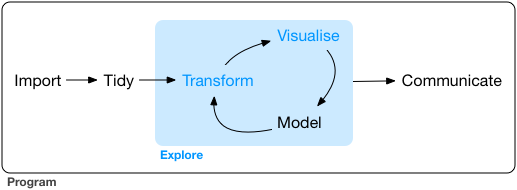
\includegraphics[width=0.8\linewidth]{/Users/Arthur/GitRepos/Teaching/data_science/boot-camp/images/data-science-explore} \end{center}

\emph{Data}: acquiring, organizing, managing, curating data (= symbols representing some measurements about the world); reformating and staging data to make it ready for analysis.
- In practice, these activities absorb \textasciitilde{} 80\% of the time of a working data scientist. (Your best friend is a good data manager!)
- Hence the value of \emph{data standards}: the more consistency in the way \emph{meaning} is represented in data, the less time, tedium, and expense spent on data mapping and transformations.

\emph{Analytics}: statistics, machine learning, modeling, other techniques for extracting summary intelligence from data.
- In general, data science practitioners don't work on developing new techniques, nor on writing code to efficiently implement techniques. Those are specializations. Most of the work involves identifying the appropriate techniques, and the right software to implement those techniques, given the data and the goals. In some cases, work will be done in close collaboration with domain area specialists, e.g., climate scientists.

\emph{Communications}: creating visualizations, narratives, etc., to reveal complexity, to convey insights. Also includes the creation of reports, dashboards, other \emph{data products}.

Doing data science requires a mix of skills: computing; statistics and other analytics; visual design and communications.

\hypertarget{data-science-projects-and-products}{%
\section{Data science projects and products}\label{data-science-projects-and-products}}

The overall mission of the Cooper Center is to leverage the resources of UVA in public service to Virginia and beyond. We have a particular focus on providing assistance to state and local officials, and to other community stakeholders. A substantial share of this work involves generating and delivering insights based on analysis of data.

\hypertarget{decision-tools-and-dashboards}{%
\subsection{Decision tools and dashboards}\label{decision-tools-and-dashboards}}

The DMME Dashboard

The SolTax tool; the SolDev tool

CTE Trailblazers dashboards: growth; gaps

\hypertarget{publications}{%
\subsection{Publications}\label{publications}}

Virginia decarbonization studies

Virginia Local Tax Rates survey

Virginia Energy Almanac

CTE Trailblazers publications: cluster briefs, longer reports

Academic publications

Student-led projects and publications

\hypertarget{research}{%
\subsection{Research}\label{research}}

Energy systems modeling

Virginia Paid Family and Medical Leave analysis

Many others, including those in collaboration with colleagues across UVA and beyond:
* Hurricane evacuation (with Engineering)
* Negative emissions
* Carbon sequestration risks
* \ldots{}

\hypertarget{shared-resources}{%
\section{Shared resources}\label{shared-resources}}

Our organization site on Github

Code base:
* Code for data cleaning and preparation
* Code for data visualization

Databases: PostgreSQL database; MySQL database; collections of flat files

Share files and folders - generally, project-specific: Box; OneDrive

Remote file storage

Slack

\emph{Cogito, ergo Zoom.}

(Email? Not so much.)

\hypertarget{working-collaboratively-in-a-team}{%
\section{Working collaboratively in a team}\label{working-collaboratively-in-a-team}}

When working on a personal project, such as a student assignment, it is typically not so necessary to assure that others can access, learn from, critique, reproduce, and build on your work.

In a team setting, it is mandatory.

We have adopted tools, processes, workflows to try to assure that your own work can be used by others, and vice versa.

\hypertarget{reproducible-workflows}{%
\section{Reproducible workflows}\label{reproducible-workflows}}

Essential for us that workflows be \emph{reproducible}, auditable, transparent.

\hypertarget{the-concept-of-reproducibility}{%
\subsection{The concept of reproducibility}\label{the-concept-of-reproducibility}}

Idea: when you present your results, you present \emph{all} of the data and the code that another practitioner (of reasonable skill) would need to reproduce your work.\footnote{We distinguish \emph{reproducibility} versus \emph{replicability}. Your work is \emph{reproducible} if someone else can regenerate exactly your same results, using your data and your code. Your research results are \emph{replicable} if another researcher can get essentially the same results when applying your techniques to different but comparable data.}

We are very much a ``reproducible workflow'' shop. In ideal practice this means:

\begin{itemize}
\item
  If you generate a report or other data product, you should be able to reproduce it entirely by re-running your code. If you were to delete your report, you should be able to regenerate it exactly, simply by re-running your code. This process should require no manual inputs from you, no cutting-and-pasting.
\item
  If you provide someone else with your code and your data, they should be able to reproduce your report by running your code on their machine. This should be true even if they are using a different type of machine, with a different operating system and directory structure. They should not need to edit your code, make manual inputs, or perform any cut-and-paste operations.
\end{itemize}

\hypertarget{how-we-create-reproducibility-in-practice}{%
\subsection{How we create reproducibility in practice}\label{how-we-create-reproducibility-in-practice}}

These conditions are ideals. In practice, we want to get as close as we can, within reason. Many of the tools that we use, and work processes we adopt, are designed to make our workflows hew closely to this ideal of full reproducibility.

R Markdown is designed specifically to enable the generation of reports and other products reproducibly.

Git and Github enable frequent backup of code and other files, and collaboration between colleagues without losing version control.

Cloud servers for maintaining files and databases help assure that our work is available to each other, properly backed up and curated, and organized in a structured way to facilitate reuse, without loss of version control.

We seek to avoid as much as possible exchanges of the form, ``I don't know why my code won't work on your machine. It runs just fine on mine!''

In particular: except possibly in the course of single work session, you should never have work-related data or code that exists only on your own machine. Ever. Your work, including data and code, should always be backed up to resources that are accessible by other team members.

\hypertarget{data-pipelines}{%
\chapter{Data pipelines}\label{data-pipelines}}

\hypertarget{retrieving-data}{%
\section{Retrieving data}\label{retrieving-data}}

\hypertarget{from-local-files}{%
\subsection{From local files}\label{from-local-files}}

\hypertarget{from-apis}{%
\subsection{From APIs}\label{from-apis}}

\hypertarget{from-databases}{%
\subsection{From databases}\label{from-databases}}

Instructions for database access

\begin{enumerate}
\def\labelenumi{(\arabic{enumi})}
\tightlist
\item
  Install DBeaver (unless you already have desktop database client software you prefer): Here is a link to download for both Windows and Mac OS X. We will be using the community edition 7.0.0. for accessing PostgreSQL databases.
\end{enumerate}

The Community Edition is free. Note that DBeaver uses and requires Java. If you install it via the Windows or MacOS installer then you don't need to install Java separately.

\begin{enumerate}
\def\labelenumi{(\arabic{enumi})}
\setcounter{enumi}{1}
\tightlist
\item
  Download and install Cisco Mobility VPN client: See instructions here.
\end{enumerate}

After launch, select the ``UVA Anywhere'' network.

You need to use the VPN if and only if you are access the database from off-Grounds. When you are on-Grounds, skip this step.

\begin{enumerate}
\def\labelenumi{(\arabic{enumi})}
\setcounter{enumi}{2}
\item
  Log into Postgres DB:

  Host: va-energy2.postgres.database.azure.com
  Username: {[}your UVA id{]}\citet{va-energy2}
  Password: {[}Contact Chloe Fauvel Chloe to get your individual password{]}
  Port: 5432
  Initial database: postgres
\end{enumerate}

Please don't share your individual credentials.

\hypertarget{from-web-resources}{%
\subsection{From web resources}\label{from-web-resources}}

\hypertarget{data-types}{%
\section{Data types}\label{data-types}}

\hypertarget{data-types-in-r}{%
\subsection{Data types in R}\label{data-types-in-r}}

\hypertarget{conversion-on-read-in}{%
\subsection{Conversion on read-in}\label{conversion-on-read-in}}

\hypertarget{data-wrangling}{%
\section{Data wrangling}\label{data-wrangling}}

To learn how to wrangle and visualize data using the Tidyverse packages, you may find it useful to go through the \href{https://learn.datacamp.com/skill-tracks/tidyverse-fundamentals}{Tidyverse Fundamentals with R} modules on \href{https://learn.datacamp.com/}{Datacamp}.
- Datacamp also offers \href{https://learn.datacamp.com/career-tracks/data-scientist-with-r}{a range of other learning modules for developing data science skills in R}.

\hypertarget{tidy-data}{%
\subsection{Tidy data}\label{tidy-data}}

\hypertarget{dplyr}{%
\subsection{Dplyr}\label{dplyr}}

\hypertarget{managing-data}{%
\section{Managing data}\label{managing-data}}

\hypertarget{dos-and-donts}{%
\subsection{DOs and DON'Ts}\label{dos-and-donts}}

\hypertarget{data-wrangling-1}{%
\chapter{Data wrangling}\label{data-wrangling-1}}

To learn how to wrangle and visualize data using the Tidyverse packages, you may find it useful to go through the \href{https://learn.datacamp.com/skill-tracks/tidyverse-fundamentals}{Tidyverse Fundamentals with R} modules on \href{https://learn.datacamp.com/}{Datacamp}.

Datacamp also offers \href{https://learn.datacamp.com/career-tracks/data-scientist-with-r}{a range of other learning modules for developing data science skills in R}.

\hypertarget{tidy-data-1}{%
\section{Tidy data}\label{tidy-data-1}}

\hypertarget{dplyr-1}{%
\section{Dplyr}\label{dplyr-1}}

\hypertarget{managing-data-1}{%
\section{Managing data}\label{managing-data-1}}

\hypertarget{dos-and-donts-1}{%
\subsection{DOs and DON'Ts}\label{dos-and-donts-1}}

\hypertarget{git-and-github-1}{%
\chapter{Git and Github}\label{git-and-github-1}}

A collection of files associated with a single project is in git-speak called a ``repository'' or \emph{``repo''}.

Depending on your project, there may already be one or more repos on Github that you will work on. The next step is to copy (``clone'') this remote repo to your local machine.

\begin{itemize}
\tightlist
\item
  Clone your course repo on Github to a new R Studio project on your local machine.

  \begin{itemize}
  \tightlist
  \item
    Navigate to \href{https://github.com/uva-eng-time-series-sp21}{the course website on Github}. Select your repo.
  \item
    Click on the green button labeled ``Code''. Copy the URL.
  \item
    In the R Studio window, from the pull-down menu in the upper-right corner, select \texttt{New\ Project...}, \texttt{Version\ Control}, \texttt{Git}. Paste the URL into the dialog box labeled \texttt{Repository\ URL}.
  \item
    Optional: Change the name of the project folder, and the location of this folder on your local directory tree.
  \item
    Click on \texttt{Create\ Project}. The files from your remote repo should be copied to your local machine in a new folder with the name you chose.
  \end{itemize}
\end{itemize}

\hypertarget{version-control-what-and-why}{%
\section{Version control: what and why}\label{version-control-what-and-why}}

\hypertarget{how-git-works}{%
\section{How git works}\label{how-git-works}}

\hypertarget{the-.gitignore-file}{%
\subsection{The .gitignore file}\label{the-.gitignore-file}}

\hypertarget{git-in-r-studio}{%
\section{Git in R Studio}\label{git-in-r-studio}}

\hypertarget{github}{%
\section{Github}\label{github}}

\hypertarget{using-personal-tokens-to-access-github}{%
\subsection{Using personal tokens to access Github}\label{using-personal-tokens-to-access-github}}

Github is phasing out the use of passwords for authorizations.

\begin{verbatim}
---- Forwarded Message -----
From: GitHub <noreply@github.com>
To: Arthur Small <asmall@virginia.edu>
Sent: Sunday, February 21, 2021, 6:20:58 AM EST
Subject: [GitHub] Deprecation Notice

Hi @arthursmalliii,

You recently used a password to access the repository at uva-eng-time-series-sp21/coronato-nicholas with git using git/2.30.0.

Basic authentication using a password to Git is deprecated and will soon no longer work. Visit https://github.blog/2020-12-15-token-authentication-requirements-for-git-operations/ for more information around suggested workarounds and removal dates.

Thanks,
The GitHub Team
\end{verbatim}

Instead, you must create a personal access token. See the Github documentation.
\#\# The Cooper Center Organization on Github

\hypertarget{best-practices}{%
\section{Best practices}\label{best-practices}}

\hypertarget{r-markdown}{%
\chapter{R Markdown}\label{r-markdown}}

Markdown is a markup language: a set of formatting instructions for rendering documents. R Markdown is an extension of Markdown that allows for embedding chunks of R code into a Markdown document. In this course, we will write our work in R Markdown within the R Studio environment, then use the \texttt{knitr} package to generate HTML and PDF output files.

For a nice introduction to Markdown and R Markdown, watch the short YouTube video \href{https://www.youtube.com/watch?v=ZzDSkBgt9xQ}{Reproducible Reports with R Markdown (STAT 545 Episode 3-A)} from the University of British Columbia.

As you proceed in creating your documents, you will probably want to access additional resources:

\begin{itemize}
\item
  From within R Studio, you can access an R Markdown Cheat Sheet via \texttt{Help/Cheatsheets}.
\item
  Markdown reference: \url{https://www.markdownguide.org/}
\item
  R Markdown reference: \url{https://rmarkdown.rstudio.com/}
\end{itemize}

\hypertarget{shared-resources-1}{%
\chapter{Shared resources}\label{shared-resources-1}}

\hypertarget{network-file-server}{%
\section{Network File Server}\label{network-file-server}}

\hypertarget{instructions-for-mounting-network-file-server-on-your-own-machine}{%
\subsection{Instructions for mounting network file server on your own machine}\label{instructions-for-mounting-network-file-server-on-your-own-machine}}

For sharing certain files, especially larger data files, the project uses a 200 GB Premium network file server (NFS) hosted by UVA Information Technology Services. This network file server is pre-mounted on the project virtual machine, making the files available to all team members. If you are doing your work on a VM, you are all set: you don't need these instructions.

It sometimes can be useful to be able to access the NFS directly from your own machine, outside the VM. The instructions here tell you how to mount the NFS on your own local machine.

Credentials and network access:
To access the NFS, you must be a member of the ceps-cleanenergyva group registered with UVA ITS. If you encounter a permissions issue when trying to access the NFS, check mygroups.virginia.edu to confirm you are a member of ceps-cleanenergyva; if you are not, contact Chloe Fauvel Chloe, David Hill David, or Arthur Small Arthur to request you be added.
To access the NFS, you must be logged on to the UVA Anywhere network. If you are off-Grounds, you will need to access the UVA Anywhere network using a VPN. If you are physically on Grounds, you should have access automatically.

{[}INSERT HERE: Instructions for mounting NFS on Windows, Mac.{]}

\hypertarget{bibliographic-resources}{%
\chapter{Bibliographic resources}\label{bibliographic-resources}}

\hypertarget{zotero}{%
\section{Zotero}\label{zotero}}

\hypertarget{bibtex}{%
\section{Bibtex}\label{bibtex}}

  \bibliography{book.bib,packages.bib}

\end{document}
